\documentclass[11pt]{article}

    \usepackage[breakable]{tcolorbox}
    \usepackage{parskip} % Stop auto-indenting (to mimic markdown behaviour)
    
    \usepackage{iftex}
    \ifPDFTeX
    	\usepackage[T1]{fontenc}
    	\usepackage{mathpazo}
    \else
    	\usepackage{fontspec}
    \fi

    % Basic figure setup, for now with no caption control since it's done
    % automatically by Pandoc (which extracts ![](path) syntax from Markdown).
    \usepackage{graphicx}
    % Maintain compatibility with old templates. Remove in nbconvert 6.0
    \let\Oldincludegraphics\includegraphics
    % Ensure that by default, figures have no caption (until we provide a
    % proper Figure object with a Caption API and a way to capture that
    % in the conversion process - todo).
    \usepackage{caption}
    \DeclareCaptionFormat{nocaption}{}
    \captionsetup{format=nocaption,aboveskip=0pt,belowskip=0pt}

    \usepackage{float}
    \floatplacement{figure}{H} % forces figures to be placed at the correct location
    \usepackage{xcolor} % Allow colors to be defined
    \usepackage{enumerate} % Needed for markdown enumerations to work
    \usepackage{geometry} % Used to adjust the document margins
    \usepackage{amsmath} % Equations
    \usepackage{amssymb} % Equations
    \usepackage{textcomp} % defines textquotesingle
    % Hack from http://tex.stackexchange.com/a/47451/13684:
    \AtBeginDocument{%
        \def\PYZsq{\textquotesingle}% Upright quotes in Pygmentized code
    }
    \usepackage{upquote} % Upright quotes for verbatim code
    \usepackage{eurosym} % defines \euro
    \usepackage[mathletters]{ucs} % Extended unicode (utf-8) support
    \usepackage{fancyvrb} % verbatim replacement that allows latex
    \usepackage{grffile} % extends the file name processing of package graphics 
                         % to support a larger range
    \makeatletter % fix for old versions of grffile with XeLaTeX
    \@ifpackagelater{grffile}{2019/11/01}
    {
      % Do nothing on new versions
    }
    {
      \def\Gread@@xetex#1{%
        \IfFileExists{"\Gin@base".bb}%
        {\Gread@eps{\Gin@base.bb}}%
        {\Gread@@xetex@aux#1}%
      }
    }
    \makeatother
    \usepackage[Export]{adjustbox} % Used to constrain images to a maximum size
    \adjustboxset{max size={0.9\linewidth}{0.9\paperheight}}

    % The hyperref package gives us a pdf with properly built
    % internal navigation ('pdf bookmarks' for the table of contents,
    % internal cross-reference links, web links for URLs, etc.)
    \usepackage{hyperref}
    % The default LaTeX title has an obnoxious amount of whitespace. By default,
    % titling removes some of it. It also provides customization options.
    \usepackage{titling}
    \usepackage{longtable} % longtable support required by pandoc >1.10
    \usepackage{booktabs}  % table support for pandoc > 1.12.2
    \usepackage[inline]{enumitem} % IRkernel/repr support (it uses the enumerate* environment)
    \usepackage[normalem]{ulem} % ulem is needed to support strikethroughs (\sout)
                                % normalem makes italics be italics, not underlines
    \usepackage{mathrsfs}
    

    
    % Colors for the hyperref package
    \definecolor{urlcolor}{rgb}{0,.145,.698}
    \definecolor{linkcolor}{rgb}{.71,0.21,0.01}
    \definecolor{citecolor}{rgb}{.12,.54,.11}

    % ANSI colors
    \definecolor{ansi-black}{HTML}{3E424D}
    \definecolor{ansi-black-intense}{HTML}{282C36}
    \definecolor{ansi-red}{HTML}{E75C58}
    \definecolor{ansi-red-intense}{HTML}{B22B31}
    \definecolor{ansi-green}{HTML}{00A250}
    \definecolor{ansi-green-intense}{HTML}{007427}
    \definecolor{ansi-yellow}{HTML}{DDB62B}
    \definecolor{ansi-yellow-intense}{HTML}{B27D12}
    \definecolor{ansi-blue}{HTML}{208FFB}
    \definecolor{ansi-blue-intense}{HTML}{0065CA}
    \definecolor{ansi-magenta}{HTML}{D160C4}
    \definecolor{ansi-magenta-intense}{HTML}{A03196}
    \definecolor{ansi-cyan}{HTML}{60C6C8}
    \definecolor{ansi-cyan-intense}{HTML}{258F8F}
    \definecolor{ansi-white}{HTML}{C5C1B4}
    \definecolor{ansi-white-intense}{HTML}{A1A6B2}
    \definecolor{ansi-default-inverse-fg}{HTML}{FFFFFF}
    \definecolor{ansi-default-inverse-bg}{HTML}{000000}

    % common color for the border for error outputs.
    \definecolor{outerrorbackground}{HTML}{FFDFDF}

    % commands and environments needed by pandoc snippets
    % extracted from the output of `pandoc -s`
    \providecommand{\tightlist}{%
      \setlength{\itemsep}{0pt}\setlength{\parskip}{0pt}}
    \DefineVerbatimEnvironment{Highlighting}{Verbatim}{commandchars=\\\{\}}
    % Add ',fontsize=\small' for more characters per line
    \newenvironment{Shaded}{}{}
    \newcommand{\KeywordTok}[1]{\textcolor[rgb]{0.00,0.44,0.13}{\textbf{{#1}}}}
    \newcommand{\DataTypeTok}[1]{\textcolor[rgb]{0.56,0.13,0.00}{{#1}}}
    \newcommand{\DecValTok}[1]{\textcolor[rgb]{0.25,0.63,0.44}{{#1}}}
    \newcommand{\BaseNTok}[1]{\textcolor[rgb]{0.25,0.63,0.44}{{#1}}}
    \newcommand{\FloatTok}[1]{\textcolor[rgb]{0.25,0.63,0.44}{{#1}}}
    \newcommand{\CharTok}[1]{\textcolor[rgb]{0.25,0.44,0.63}{{#1}}}
    \newcommand{\StringTok}[1]{\textcolor[rgb]{0.25,0.44,0.63}{{#1}}}
    \newcommand{\CommentTok}[1]{\textcolor[rgb]{0.38,0.63,0.69}{\textit{{#1}}}}
    \newcommand{\OtherTok}[1]{\textcolor[rgb]{0.00,0.44,0.13}{{#1}}}
    \newcommand{\AlertTok}[1]{\textcolor[rgb]{1.00,0.00,0.00}{\textbf{{#1}}}}
    \newcommand{\FunctionTok}[1]{\textcolor[rgb]{0.02,0.16,0.49}{{#1}}}
    \newcommand{\RegionMarkerTok}[1]{{#1}}
    \newcommand{\ErrorTok}[1]{\textcolor[rgb]{1.00,0.00,0.00}{\textbf{{#1}}}}
    \newcommand{\NormalTok}[1]{{#1}}
    
    % Additional commands for more recent versions of Pandoc
    \newcommand{\ConstantTok}[1]{\textcolor[rgb]{0.53,0.00,0.00}{{#1}}}
    \newcommand{\SpecialCharTok}[1]{\textcolor[rgb]{0.25,0.44,0.63}{{#1}}}
    \newcommand{\VerbatimStringTok}[1]{\textcolor[rgb]{0.25,0.44,0.63}{{#1}}}
    \newcommand{\SpecialStringTok}[1]{\textcolor[rgb]{0.73,0.40,0.53}{{#1}}}
    \newcommand{\ImportTok}[1]{{#1}}
    \newcommand{\DocumentationTok}[1]{\textcolor[rgb]{0.73,0.13,0.13}{\textit{{#1}}}}
    \newcommand{\AnnotationTok}[1]{\textcolor[rgb]{0.38,0.63,0.69}{\textbf{\textit{{#1}}}}}
    \newcommand{\CommentVarTok}[1]{\textcolor[rgb]{0.38,0.63,0.69}{\textbf{\textit{{#1}}}}}
    \newcommand{\VariableTok}[1]{\textcolor[rgb]{0.10,0.09,0.49}{{#1}}}
    \newcommand{\ControlFlowTok}[1]{\textcolor[rgb]{0.00,0.44,0.13}{\textbf{{#1}}}}
    \newcommand{\OperatorTok}[1]{\textcolor[rgb]{0.40,0.40,0.40}{{#1}}}
    \newcommand{\BuiltInTok}[1]{{#1}}
    \newcommand{\ExtensionTok}[1]{{#1}}
    \newcommand{\PreprocessorTok}[1]{\textcolor[rgb]{0.74,0.48,0.00}{{#1}}}
    \newcommand{\AttributeTok}[1]{\textcolor[rgb]{0.49,0.56,0.16}{{#1}}}
    \newcommand{\InformationTok}[1]{\textcolor[rgb]{0.38,0.63,0.69}{\textbf{\textit{{#1}}}}}
    \newcommand{\WarningTok}[1]{\textcolor[rgb]{0.38,0.63,0.69}{\textbf{\textit{{#1}}}}}
    
    
    % Define a nice break command that doesn't care if a line doesn't already
    % exist.
    \def\br{\hspace*{\fill} \\* }
    % Math Jax compatibility definitions
    \def\gt{>}
    \def\lt{<}
    \let\Oldtex\TeX
    \let\Oldlatex\LaTeX
    \renewcommand{\TeX}{\textrm{\Oldtex}}
    \renewcommand{\LaTeX}{\textrm{\Oldlatex}}
    % Document parameters
    % Document title
    \title{A\_Bayesian\_Model\_For\_News\_Reporting}
    
    
    
    
    
% Pygments definitions
\makeatletter
\def\PY@reset{\let\PY@it=\relax \let\PY@bf=\relax%
    \let\PY@ul=\relax \let\PY@tc=\relax%
    \let\PY@bc=\relax \let\PY@ff=\relax}
\def\PY@tok#1{\csname PY@tok@#1\endcsname}
\def\PY@toks#1+{\ifx\relax#1\empty\else%
    \PY@tok{#1}\expandafter\PY@toks\fi}
\def\PY@do#1{\PY@bc{\PY@tc{\PY@ul{%
    \PY@it{\PY@bf{\PY@ff{#1}}}}}}}
\def\PY#1#2{\PY@reset\PY@toks#1+\relax+\PY@do{#2}}

\@namedef{PY@tok@w}{\def\PY@tc##1{\textcolor[rgb]{0.73,0.73,0.73}{##1}}}
\@namedef{PY@tok@c}{\let\PY@it=\textit\def\PY@tc##1{\textcolor[rgb]{0.25,0.50,0.50}{##1}}}
\@namedef{PY@tok@cp}{\def\PY@tc##1{\textcolor[rgb]{0.74,0.48,0.00}{##1}}}
\@namedef{PY@tok@k}{\let\PY@bf=\textbf\def\PY@tc##1{\textcolor[rgb]{0.00,0.50,0.00}{##1}}}
\@namedef{PY@tok@kp}{\def\PY@tc##1{\textcolor[rgb]{0.00,0.50,0.00}{##1}}}
\@namedef{PY@tok@kt}{\def\PY@tc##1{\textcolor[rgb]{0.69,0.00,0.25}{##1}}}
\@namedef{PY@tok@o}{\def\PY@tc##1{\textcolor[rgb]{0.40,0.40,0.40}{##1}}}
\@namedef{PY@tok@ow}{\let\PY@bf=\textbf\def\PY@tc##1{\textcolor[rgb]{0.67,0.13,1.00}{##1}}}
\@namedef{PY@tok@nb}{\def\PY@tc##1{\textcolor[rgb]{0.00,0.50,0.00}{##1}}}
\@namedef{PY@tok@nf}{\def\PY@tc##1{\textcolor[rgb]{0.00,0.00,1.00}{##1}}}
\@namedef{PY@tok@nc}{\let\PY@bf=\textbf\def\PY@tc##1{\textcolor[rgb]{0.00,0.00,1.00}{##1}}}
\@namedef{PY@tok@nn}{\let\PY@bf=\textbf\def\PY@tc##1{\textcolor[rgb]{0.00,0.00,1.00}{##1}}}
\@namedef{PY@tok@ne}{\let\PY@bf=\textbf\def\PY@tc##1{\textcolor[rgb]{0.82,0.25,0.23}{##1}}}
\@namedef{PY@tok@nv}{\def\PY@tc##1{\textcolor[rgb]{0.10,0.09,0.49}{##1}}}
\@namedef{PY@tok@no}{\def\PY@tc##1{\textcolor[rgb]{0.53,0.00,0.00}{##1}}}
\@namedef{PY@tok@nl}{\def\PY@tc##1{\textcolor[rgb]{0.63,0.63,0.00}{##1}}}
\@namedef{PY@tok@ni}{\let\PY@bf=\textbf\def\PY@tc##1{\textcolor[rgb]{0.60,0.60,0.60}{##1}}}
\@namedef{PY@tok@na}{\def\PY@tc##1{\textcolor[rgb]{0.49,0.56,0.16}{##1}}}
\@namedef{PY@tok@nt}{\let\PY@bf=\textbf\def\PY@tc##1{\textcolor[rgb]{0.00,0.50,0.00}{##1}}}
\@namedef{PY@tok@nd}{\def\PY@tc##1{\textcolor[rgb]{0.67,0.13,1.00}{##1}}}
\@namedef{PY@tok@s}{\def\PY@tc##1{\textcolor[rgb]{0.73,0.13,0.13}{##1}}}
\@namedef{PY@tok@sd}{\let\PY@it=\textit\def\PY@tc##1{\textcolor[rgb]{0.73,0.13,0.13}{##1}}}
\@namedef{PY@tok@si}{\let\PY@bf=\textbf\def\PY@tc##1{\textcolor[rgb]{0.73,0.40,0.53}{##1}}}
\@namedef{PY@tok@se}{\let\PY@bf=\textbf\def\PY@tc##1{\textcolor[rgb]{0.73,0.40,0.13}{##1}}}
\@namedef{PY@tok@sr}{\def\PY@tc##1{\textcolor[rgb]{0.73,0.40,0.53}{##1}}}
\@namedef{PY@tok@ss}{\def\PY@tc##1{\textcolor[rgb]{0.10,0.09,0.49}{##1}}}
\@namedef{PY@tok@sx}{\def\PY@tc##1{\textcolor[rgb]{0.00,0.50,0.00}{##1}}}
\@namedef{PY@tok@m}{\def\PY@tc##1{\textcolor[rgb]{0.40,0.40,0.40}{##1}}}
\@namedef{PY@tok@gh}{\let\PY@bf=\textbf\def\PY@tc##1{\textcolor[rgb]{0.00,0.00,0.50}{##1}}}
\@namedef{PY@tok@gu}{\let\PY@bf=\textbf\def\PY@tc##1{\textcolor[rgb]{0.50,0.00,0.50}{##1}}}
\@namedef{PY@tok@gd}{\def\PY@tc##1{\textcolor[rgb]{0.63,0.00,0.00}{##1}}}
\@namedef{PY@tok@gi}{\def\PY@tc##1{\textcolor[rgb]{0.00,0.63,0.00}{##1}}}
\@namedef{PY@tok@gr}{\def\PY@tc##1{\textcolor[rgb]{1.00,0.00,0.00}{##1}}}
\@namedef{PY@tok@ge}{\let\PY@it=\textit}
\@namedef{PY@tok@gs}{\let\PY@bf=\textbf}
\@namedef{PY@tok@gp}{\let\PY@bf=\textbf\def\PY@tc##1{\textcolor[rgb]{0.00,0.00,0.50}{##1}}}
\@namedef{PY@tok@go}{\def\PY@tc##1{\textcolor[rgb]{0.53,0.53,0.53}{##1}}}
\@namedef{PY@tok@gt}{\def\PY@tc##1{\textcolor[rgb]{0.00,0.27,0.87}{##1}}}
\@namedef{PY@tok@err}{\def\PY@bc##1{{\setlength{\fboxsep}{\string -\fboxrule}\fcolorbox[rgb]{1.00,0.00,0.00}{1,1,1}{\strut ##1}}}}
\@namedef{PY@tok@kc}{\let\PY@bf=\textbf\def\PY@tc##1{\textcolor[rgb]{0.00,0.50,0.00}{##1}}}
\@namedef{PY@tok@kd}{\let\PY@bf=\textbf\def\PY@tc##1{\textcolor[rgb]{0.00,0.50,0.00}{##1}}}
\@namedef{PY@tok@kn}{\let\PY@bf=\textbf\def\PY@tc##1{\textcolor[rgb]{0.00,0.50,0.00}{##1}}}
\@namedef{PY@tok@kr}{\let\PY@bf=\textbf\def\PY@tc##1{\textcolor[rgb]{0.00,0.50,0.00}{##1}}}
\@namedef{PY@tok@bp}{\def\PY@tc##1{\textcolor[rgb]{0.00,0.50,0.00}{##1}}}
\@namedef{PY@tok@fm}{\def\PY@tc##1{\textcolor[rgb]{0.00,0.00,1.00}{##1}}}
\@namedef{PY@tok@vc}{\def\PY@tc##1{\textcolor[rgb]{0.10,0.09,0.49}{##1}}}
\@namedef{PY@tok@vg}{\def\PY@tc##1{\textcolor[rgb]{0.10,0.09,0.49}{##1}}}
\@namedef{PY@tok@vi}{\def\PY@tc##1{\textcolor[rgb]{0.10,0.09,0.49}{##1}}}
\@namedef{PY@tok@vm}{\def\PY@tc##1{\textcolor[rgb]{0.10,0.09,0.49}{##1}}}
\@namedef{PY@tok@sa}{\def\PY@tc##1{\textcolor[rgb]{0.73,0.13,0.13}{##1}}}
\@namedef{PY@tok@sb}{\def\PY@tc##1{\textcolor[rgb]{0.73,0.13,0.13}{##1}}}
\@namedef{PY@tok@sc}{\def\PY@tc##1{\textcolor[rgb]{0.73,0.13,0.13}{##1}}}
\@namedef{PY@tok@dl}{\def\PY@tc##1{\textcolor[rgb]{0.73,0.13,0.13}{##1}}}
\@namedef{PY@tok@s2}{\def\PY@tc##1{\textcolor[rgb]{0.73,0.13,0.13}{##1}}}
\@namedef{PY@tok@sh}{\def\PY@tc##1{\textcolor[rgb]{0.73,0.13,0.13}{##1}}}
\@namedef{PY@tok@s1}{\def\PY@tc##1{\textcolor[rgb]{0.73,0.13,0.13}{##1}}}
\@namedef{PY@tok@mb}{\def\PY@tc##1{\textcolor[rgb]{0.40,0.40,0.40}{##1}}}
\@namedef{PY@tok@mf}{\def\PY@tc##1{\textcolor[rgb]{0.40,0.40,0.40}{##1}}}
\@namedef{PY@tok@mh}{\def\PY@tc##1{\textcolor[rgb]{0.40,0.40,0.40}{##1}}}
\@namedef{PY@tok@mi}{\def\PY@tc##1{\textcolor[rgb]{0.40,0.40,0.40}{##1}}}
\@namedef{PY@tok@il}{\def\PY@tc##1{\textcolor[rgb]{0.40,0.40,0.40}{##1}}}
\@namedef{PY@tok@mo}{\def\PY@tc##1{\textcolor[rgb]{0.40,0.40,0.40}{##1}}}
\@namedef{PY@tok@ch}{\let\PY@it=\textit\def\PY@tc##1{\textcolor[rgb]{0.25,0.50,0.50}{##1}}}
\@namedef{PY@tok@cm}{\let\PY@it=\textit\def\PY@tc##1{\textcolor[rgb]{0.25,0.50,0.50}{##1}}}
\@namedef{PY@tok@cpf}{\let\PY@it=\textit\def\PY@tc##1{\textcolor[rgb]{0.25,0.50,0.50}{##1}}}
\@namedef{PY@tok@c1}{\let\PY@it=\textit\def\PY@tc##1{\textcolor[rgb]{0.25,0.50,0.50}{##1}}}
\@namedef{PY@tok@cs}{\let\PY@it=\textit\def\PY@tc##1{\textcolor[rgb]{0.25,0.50,0.50}{##1}}}

\def\PYZbs{\char`\\}
\def\PYZus{\char`\_}
\def\PYZob{\char`\{}
\def\PYZcb{\char`\}}
\def\PYZca{\char`\^}
\def\PYZam{\char`\&}
\def\PYZlt{\char`\<}
\def\PYZgt{\char`\>}
\def\PYZsh{\char`\#}
\def\PYZpc{\char`\%}
\def\PYZdl{\char`\$}
\def\PYZhy{\char`\-}
\def\PYZsq{\char`\'}
\def\PYZdq{\char`\"}
\def\PYZti{\char`\~}
% for compatibility with earlier versions
\def\PYZat{@}
\def\PYZlb{[}
\def\PYZrb{]}
\makeatother


    % For linebreaks inside Verbatim environment from package fancyvrb. 
    \makeatletter
        \newbox\Wrappedcontinuationbox 
        \newbox\Wrappedvisiblespacebox 
        \newcommand*\Wrappedvisiblespace {\textcolor{red}{\textvisiblespace}} 
        \newcommand*\Wrappedcontinuationsymbol {\textcolor{red}{\llap{\tiny$\m@th\hookrightarrow$}}} 
        \newcommand*\Wrappedcontinuationindent {3ex } 
        \newcommand*\Wrappedafterbreak {\kern\Wrappedcontinuationindent\copy\Wrappedcontinuationbox} 
        % Take advantage of the already applied Pygments mark-up to insert 
        % potential linebreaks for TeX processing. 
        %        {, <, #, %, $, ' and ": go to next line. 
        %        _, }, ^, &, >, - and ~: stay at end of broken line. 
        % Use of \textquotesingle for straight quote. 
        \newcommand*\Wrappedbreaksatspecials {% 
            \def\PYGZus{\discretionary{\char`\_}{\Wrappedafterbreak}{\char`\_}}% 
            \def\PYGZob{\discretionary{}{\Wrappedafterbreak\char`\{}{\char`\{}}% 
            \def\PYGZcb{\discretionary{\char`\}}{\Wrappedafterbreak}{\char`\}}}% 
            \def\PYGZca{\discretionary{\char`\^}{\Wrappedafterbreak}{\char`\^}}% 
            \def\PYGZam{\discretionary{\char`\&}{\Wrappedafterbreak}{\char`\&}}% 
            \def\PYGZlt{\discretionary{}{\Wrappedafterbreak\char`\<}{\char`\<}}% 
            \def\PYGZgt{\discretionary{\char`\>}{\Wrappedafterbreak}{\char`\>}}% 
            \def\PYGZsh{\discretionary{}{\Wrappedafterbreak\char`\#}{\char`\#}}% 
            \def\PYGZpc{\discretionary{}{\Wrappedafterbreak\char`\%}{\char`\%}}% 
            \def\PYGZdl{\discretionary{}{\Wrappedafterbreak\char`\$}{\char`\$}}% 
            \def\PYGZhy{\discretionary{\char`\-}{\Wrappedafterbreak}{\char`\-}}% 
            \def\PYGZsq{\discretionary{}{\Wrappedafterbreak\textquotesingle}{\textquotesingle}}% 
            \def\PYGZdq{\discretionary{}{\Wrappedafterbreak\char`\"}{\char`\"}}% 
            \def\PYGZti{\discretionary{\char`\~}{\Wrappedafterbreak}{\char`\~}}% 
        } 
        % Some characters . , ; ? ! / are not pygmentized. 
        % This macro makes them "active" and they will insert potential linebreaks 
        \newcommand*\Wrappedbreaksatpunct {% 
            \lccode`\~`\.\lowercase{\def~}{\discretionary{\hbox{\char`\.}}{\Wrappedafterbreak}{\hbox{\char`\.}}}% 
            \lccode`\~`\,\lowercase{\def~}{\discretionary{\hbox{\char`\,}}{\Wrappedafterbreak}{\hbox{\char`\,}}}% 
            \lccode`\~`\;\lowercase{\def~}{\discretionary{\hbox{\char`\;}}{\Wrappedafterbreak}{\hbox{\char`\;}}}% 
            \lccode`\~`\:\lowercase{\def~}{\discretionary{\hbox{\char`\:}}{\Wrappedafterbreak}{\hbox{\char`\:}}}% 
            \lccode`\~`\?\lowercase{\def~}{\discretionary{\hbox{\char`\?}}{\Wrappedafterbreak}{\hbox{\char`\?}}}% 
            \lccode`\~`\!\lowercase{\def~}{\discretionary{\hbox{\char`\!}}{\Wrappedafterbreak}{\hbox{\char`\!}}}% 
            \lccode`\~`\/\lowercase{\def~}{\discretionary{\hbox{\char`\/}}{\Wrappedafterbreak}{\hbox{\char`\/}}}% 
            \catcode`\.\active
            \catcode`\,\active 
            \catcode`\;\active
            \catcode`\:\active
            \catcode`\?\active
            \catcode`\!\active
            \catcode`\/\active 
            \lccode`\~`\~ 	
        }
    \makeatother

    \let\OriginalVerbatim=\Verbatim
    \makeatletter
    \renewcommand{\Verbatim}[1][1]{%
        %\parskip\z@skip
        \sbox\Wrappedcontinuationbox {\Wrappedcontinuationsymbol}%
        \sbox\Wrappedvisiblespacebox {\FV@SetupFont\Wrappedvisiblespace}%
        \def\FancyVerbFormatLine ##1{\hsize\linewidth
            \vtop{\raggedright\hyphenpenalty\z@\exhyphenpenalty\z@
                \doublehyphendemerits\z@\finalhyphendemerits\z@
                \strut ##1\strut}%
        }%
        % If the linebreak is at a space, the latter will be displayed as visible
        % space at end of first line, and a continuation symbol starts next line.
        % Stretch/shrink are however usually zero for typewriter font.
        \def\FV@Space {%
            \nobreak\hskip\z@ plus\fontdimen3\font minus\fontdimen4\font
            \discretionary{\copy\Wrappedvisiblespacebox}{\Wrappedafterbreak}
            {\kern\fontdimen2\font}%
        }%
        
        % Allow breaks at special characters using \PYG... macros.
        \Wrappedbreaksatspecials
        % Breaks at punctuation characters . , ; ? ! and / need catcode=\active 	
        \OriginalVerbatim[#1,codes*=\Wrappedbreaksatpunct]%
    }
    \makeatother

    % Exact colors from NB
    \definecolor{incolor}{HTML}{303F9F}
    \definecolor{outcolor}{HTML}{D84315}
    \definecolor{cellborder}{HTML}{CFCFCF}
    \definecolor{cellbackground}{HTML}{F7F7F7}
    
    % prompt
    \makeatletter
    \newcommand{\boxspacing}{\kern\kvtcb@left@rule\kern\kvtcb@boxsep}
    \makeatother
    \newcommand{\prompt}[4]{
        {\ttfamily\llap{{\color{#2}[#3]:\hspace{3pt}#4}}\vspace{-\baselineskip}}
    }
    

    
    % Prevent overflowing lines due to hard-to-break entities
    \sloppy 
    % Setup hyperref package
    \hypersetup{
      breaklinks=true,  % so long urls are correctly broken across lines
      colorlinks=true,
      urlcolor=urlcolor,
      linkcolor=linkcolor,
      citecolor=citecolor,
      }
    % Slightly bigger margins than the latex defaults
    
    \geometry{verbose,tmargin=1in,bmargin=1in,lmargin=1in,rmargin=1in}
    
    

\begin{document}
    
    \maketitle
    
    

    
    \hypertarget{a-bayesian-model-for-news-reporting}{%
\section*{A Bayesian Model for News
Reporting}\label{a-bayesian-model-for-news-reporting}}
\addcontentsline{toc}{section}{A Bayesian Model for News Reporting}

\emph{Nicholas Lines}

    \hypertarget{environment-setup}{%
\section{Environment Setup}\label{environment-setup}}

    \begin{tcolorbox}[breakable, size=fbox, boxrule=1pt, pad at break*=1mm,colback=cellbackground, colframe=cellborder]
\prompt{In}{incolor}{2}{\boxspacing}
\begin{Verbatim}[commandchars=\\\{\}]
\PY{o}{\PYZpc{}}\PY{k}{pylab} inline
\end{Verbatim}
\end{tcolorbox}

    \begin{Verbatim}[commandchars=\\\{\}]
Populating the interactive namespace from numpy and matplotlib
    \end{Verbatim}

    \begin{tcolorbox}[breakable, size=fbox, boxrule=1pt, pad at break*=1mm,colback=cellbackground, colframe=cellborder]
\prompt{In}{incolor}{3}{\boxspacing}
\begin{Verbatim}[commandchars=\\\{\}]
\PY{k+kn}{import} \PY{n+nn}{scipy}\PY{n+nn}{.}\PY{n+nn}{stats} \PY{k}{as} \PY{n+nn}{st}
\end{Verbatim}
\end{tcolorbox}

    \begin{tcolorbox}[breakable, size=fbox, boxrule=1pt, pad at break*=1mm,colback=cellbackground, colframe=cellborder]
\prompt{In}{incolor}{4}{\boxspacing}
\begin{Verbatim}[commandchars=\\\{\}]
\PY{k+kn}{from} \PY{n+nn}{tqdm}\PY{n+nn}{.}\PY{n+nn}{notebook} \PY{k+kn}{import} \PY{n}{tqdm}
\end{Verbatim}
\end{tcolorbox}

    \hypertarget{a-generative-model-for-news-information}{%
\section{A Generative Model for News
Information}\label{a-generative-model-for-news-information}}

We wish to model the information network by which a news reporter can
gather facts about the news topics of interest to them. While we will
use vocabulary related to the application of gathering information about
news topics, we note that this task is analagous to many other
information-gathering-and-fusion processes.

Consider a reporter who must stay informed about \(n_j\) news topics,
indexed by \(j\). The reporter cannot observe the facts related to these
news topics directly, and relies on a network of first-hand observers to
inform the reporter. This network consists of \(n_i\) observers, indexed
by \(i\), who each provide an observation at each time step \(t\) of
\(n_t\) timesteps. These observations, labeled \(o_{i,j,t}\) (for
observer \(i\) speaking about topic \(j\) at time \(t\)) are the only
information provided to the reporter.

Many techniques have been proposed to derive ``facts'' from text streams
and other media, but we will not include these steps. Instead, we will
assume that each news topic \(j\) produces a single binary ``fact''
called \(f_{j,t}\) at each time step \(t\). (For example, the sports
topic might yield facts such as ``The tigers beat the rams on
Saturday,'' which can be represented as a 1 or 0 for true or false.) The
fact is then observed by each observer. However, we wish to model the
fact that not all observers are are equally aware of all newsworthy
subjects, and not all observers will pass on their information at each
time step. Therefore, we insist on the following dependencies.

\begin{enumerate}
\def\labelenumi{\arabic{enumi}.}
\tightlist
\item
  The binary fact for each topic and each timestep is sampled from a
  Bernoulli distribution \(f_{j,t} \sim Bern(\delta_j)\) where
  \(\delta_j\sim Unif(0,1)\) represents the bias of this news topic
  toward 1-valued facts.
\item
  Whether an observer will report their observation or not is
  represented by the binary variable
  \(\tau_{i,j,t} \sim Bern(\epsilon_{i,j})\) where
  \(\epsilon_{i,j}\sim Unif(0,1)\) represents that observer's bias
  toward reporting about this news topic.
\item
  Whether an observer is well-informed about this topic's fact at time
  \(t\) is represented by the binary variable
  \(a_{i,j,t} \sim Bern(\beta_{i,j})\) where
  \(\beta_{i,j}\sim Unif(0,1)\) is a hyperparameter representing how
  well-informed the observer is on this topic on average. This
  hyperparameter is the variable of most interest for us.
\item
  Let \(\tilde{x}\) represent \texttt{not} \(x\) for a binary variable
  \(x\). We will use a uniform random binary variable
  \(r_{i,j,t} \sim Bern(0.5)\). The observer's report to the reporter is
  \[o_{i,j,t} = \tau_{i,j,t}(a_{i,j,t}f_{j,t} + \tilde{a_{i,j,t}}r_{i,j,t}) + 2\tilde{\tau_{i,j,t}},\]
  meaning that if the observer is aware and chooses to report at this
  timestep, they report the fact \(f_{j,t}\) with no alteration; if the
  observer is unaware, the observer reports 1 or 0 with equal
  probability; and if the observer chooses not to report, a 2 is
  returned, signifying that no information was passed on.
\item
  The reporter then constructs
  \[b_j = mode_i(\{o_{i,j,t} : o_{i,j,t}\neq2\})\] as an approximation
  to \(f_{j,t}\), i.e.~the reporter's best guess at the true fact.
\end{enumerate}

This model is shown in the diagram below.

    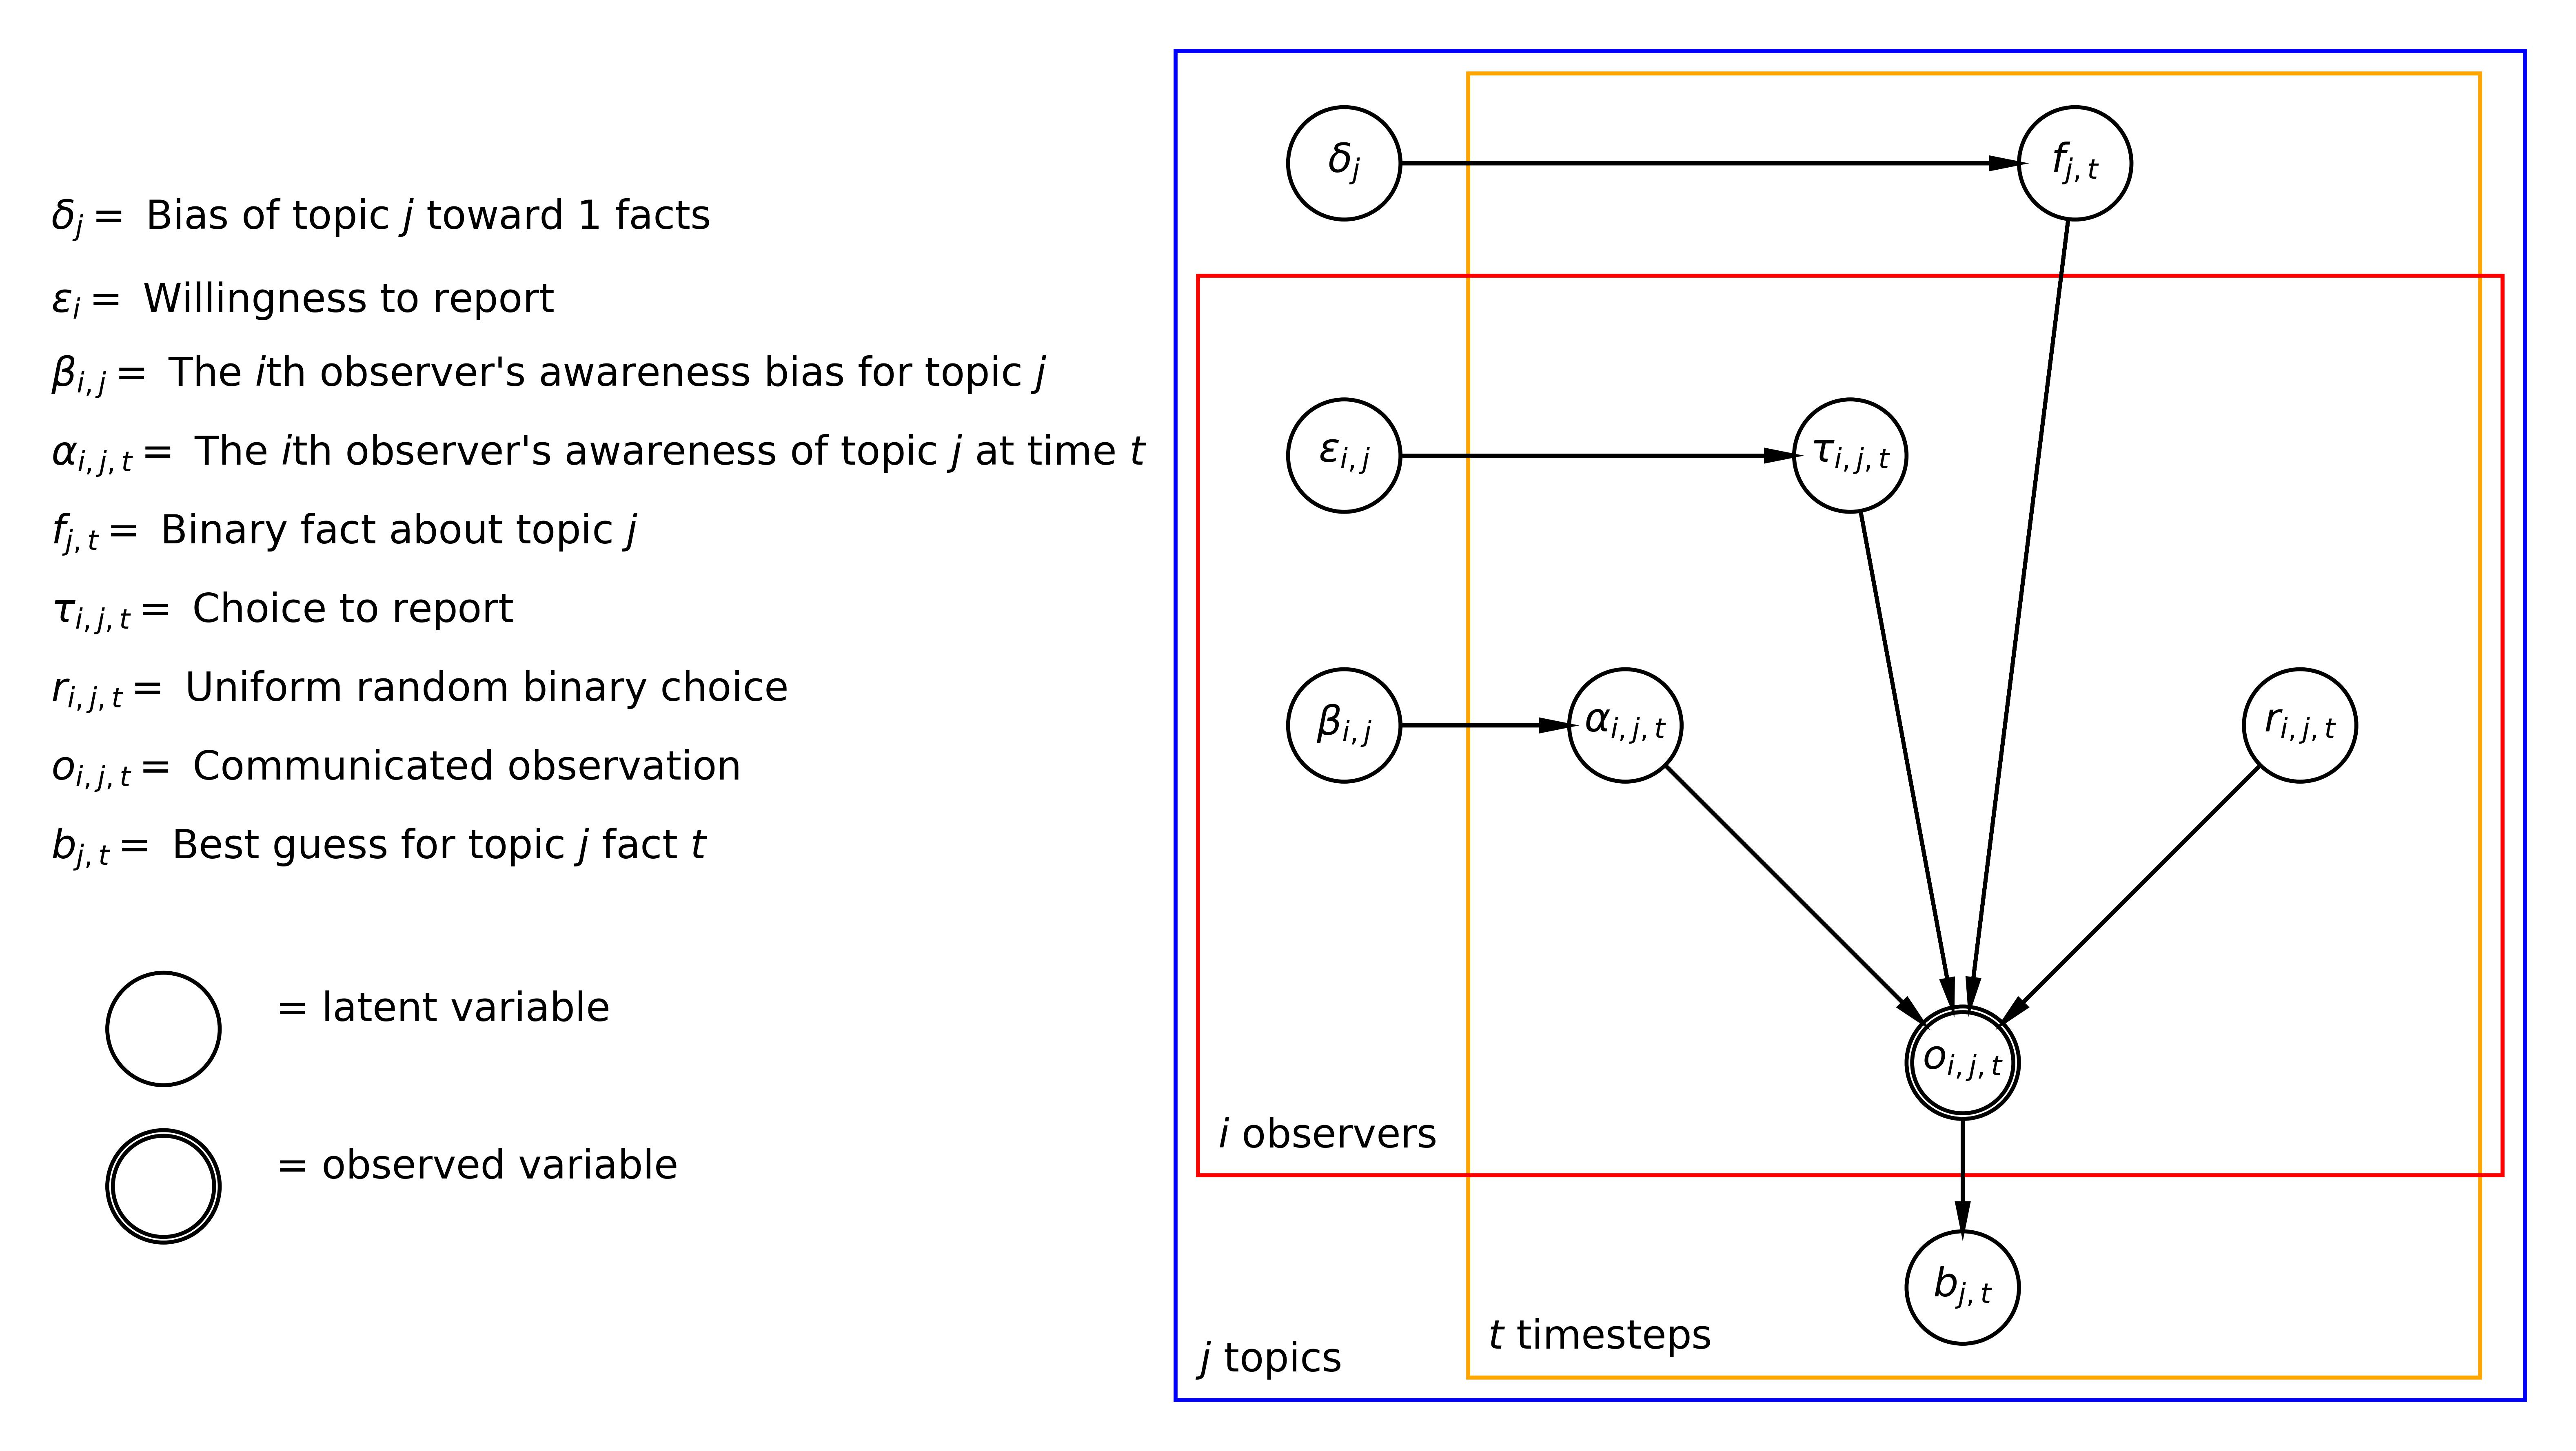
\includegraphics{../Images/reporting_network.jpg}

    We should make a few observations about this naive construction before
continuing.

\begin{enumerate}
\def\labelenumi{\arabic{enumi}.}
\tightlist
\item
  First, the approximation \(b_j \approx f_{j,t}\) is not really
  legitimate because it could well be that all observers agreed to lie.
  Really \(b_j\) tells us nothing more than the consensus of
  observations about the fact. This fact is important in situations
  where we suspect that there is not consensus or that the consensus of
  our observers is unreliable.
\item
  The model as stated leaves each topic's network entirely independent
  of the other topics, so there is no real need for the outermost plate
  in the diagram: this was included solely to remind us of this
  assumption and to indicate that this problem scales in topics \(j\).
\item
  The purpose for laying out this generative model is to help us
  strategize how to learn the observer awareness hyperparameter,
  \(\beta_{i,j}\), which will allow us to reduce the network by cutting
  all edges \(o_{i,j,t} - b_{j,t}\) when \(\beta_{i,j} < \rho\) for some
  threshold \(\rho\).
\item
  We are not interested in recovering any other hyperparameters in this
  situation. These exist solely to lend verisimilitude to the model.
\item
  If we allow \(\lvert\delta_j-0.5\rvert\) to grow too small, the
  inference problem gets much harder.
\end{enumerate}

    \hypertarget{extremely-simple-inference}{%
\section{Extremely Simple Inference}\label{extremely-simple-inference}}

Let's consider how we could approximate \(\beta_{i,j}\) using the
assumed distributions. If we condition on \(\tau_{i,j,t}=1\) we restrict
ourselves to a reveiw of the informative reports from a single observer,
i.e.~\[\{ o_{i,j,t}: o_{i,j,t}\neq 2, i=\bar{i} \},\] and we can write
\[ o_{i,j,t} = a_{i,j,t} f_{j,t} + \tilde{a}_{i,j,t} r_{i,j,t}.\]

We can quickly describe the probability distribution for \(o_{i,j,t}\)
under these conditions using a probability table (since these are all
binary variables). We recall that the parameter of each Bernoulli random
variable represents the probability that variable equals one. (For
simplicity we will drop the subscripts for the table.)

\begin{longtable}[]{@{}lllllll@{}}
\toprule
\(o\) & \(a\) & \(f\) & \(r\) & \(P(a)\) & \(P(f)\) & \(P(r)\) \\
\midrule
\endhead
0 & 1 & 0 & 0 & \(\beta\) & \(1-\delta\) & 0.5 (always) \\
1 & 1 & 1 & 0 & \(\beta\) & \(\delta\) & 0.5 \\
1 & 1 & 1 & 1 & \(\beta\) & \(\delta\) & 0.5 \\
0 & 1 & 0 & 1 & \(\beta\) & \(1-\delta\) & 0.5 \\
1 & 0 & 1 & 1 & \(1-\beta\) & \(\delta\) & 0.5 \\
1 & 0 & 0 & 1 & \(1-\beta\) & \(1-\delta\) & 0.5 \\
0 & 0 & 1 & 0 & \(1-\beta\) & \(\delta\) & 0.5 \\
0 & 0 & 0 & 0 & \(1-\beta\) & \(1-\delta\) & 0.5 \\
\bottomrule
\end{longtable}

Each of \(\beta,\delta,\) and \(r\) are mutually independent variables,
so their joint probability is the product of their marginal
probabilities. By summing up the joint probabilities of combinations
that lead us to \(o_{\bar{i},j,t}=1\) we have

\begin{align}
P(o_{\bar{i},j,t}=1) &= 0.5(\beta_{\bar{i},j}\delta_j + \delta_j - \beta_{\bar{i},j,t}\delta_j + 1 - \beta_{\bar{i},j,t} - \delta_j + \beta_{\bar{i},j,t}\delta_j + \beta_{\bar{i},j,t}\delta_j)\\
       &= 0.5(-\beta_{\bar{i},j,t} + \beta_{\bar{i},j,t}\delta_j + 1)
\end{align}

We would reach the same result with much less work using conditional
probabilities (factors), since \begin{align}
P(o_{\bar{i},j,t}=1) &= P(o_{\bar{i},j,t}=1 \mid a_{\bar{i},j,t}=0) P(a_{\bar{i},j,t}=0) + P(o_{\bar{i},j,t}=1 \mid a_{\bar{i},j,t}=1) P(a_{\bar{i},j,t}=1)\\
&= 0.5(1-\beta_{\bar{i},j}) + \delta_j \beta_{\bar{i},j}.
\end{align}

Solving for \(\beta\) gives us
\[\beta_{\bar{i},j,t} = \frac{2P(o_{\bar{i},j,t}=1) - 1}{2\delta_j - 1}.\]

    We could approximate
\[\delta_j \approx \hat{\delta_j} = \frac{ \# \{o_{i,j,t} : o_{i,j,t}=1\}}{ \# \{o_{i,j,t} : o_{i,j,t}\neq 2 \} },\]

i.e.~we use the sample mean of the informative observations to
approximate the probability that a generated fact equals 1 (an extension
of the approximation \(b_{j,t}=\hat{f}_{j,t}\approx f_{j,t}\)). But we
already have the observed mean \[\hat{\delta_j} = \bar{b_{j,t}},\] which
immediately fills that role.

Our statistic for \(P(o_{\bar{i},j,t}=1)\) is the observed probability
\[ P(o_{\bar{i},j,t}=1) = \frac{ \# \{o_{\bar{i},j,t} : o_{\bar{i},j,t}=1\}}{ \# \{o_{\bar{i},j,t} : o_{\bar{i},j,t}\neq 2 \} }.\]

Now we can make the approximation

\begin{align}
\beta_{i,j}\approx \hat{\beta_{i,j}} &= \frac{2 \frac{ \# \{o_{\bar{i},j,t} : o_{\bar{i},j,t}=1\}}{ \# \{o_{\bar{i},j,t} : o_{\bar{i},j,t}\neq 2 \} } -1}{2\hat{\delta_j}-1}\\
&= \frac{2 \frac{ \# \{o_{\bar{i},j,t} : o_{\bar{i},j,t}=1\}}{ \# \{o_{\bar{i},j,t} : o_{\bar{i},j,t}\neq 2 \} } -1}{2\frac{ \# \{o_{i,j,t} : o_{i,j,t}=1\}}{ \# \{o_{i,j,t} : o_{i,j,t}\neq 2 \} } - 1}.
\end{align}

    \hypertarget{simulating-data-with-this-model}{%
\section{Simulating Data with this
Model}\label{simulating-data-with-this-model}}

We want to create an artificial dataset so we can observe this model at
work, and hopefully show how to recover the desired hyperparameter.

    \begin{tcolorbox}[breakable, size=fbox, boxrule=1pt, pad at break*=1mm,colback=cellbackground, colframe=cellborder]
\prompt{In}{incolor}{5}{\boxspacing}
\begin{Verbatim}[commandchars=\\\{\}]
\PY{k}{def} \PY{n+nf}{bin\PYZus{}not}\PY{p}{(}\PY{n}{n}\PY{p}{)}\PY{p}{:}
    \PY{l+s+sd}{\PYZsq{}\PYZsq{}\PYZsq{}Just switch 1 and 0.\PYZsq{}\PYZsq{}\PYZsq{}}
    \PY{k}{return} \PY{l+m+mi}{1} \PY{o}{\PYZhy{}} \PY{l+m+mi}{1}\PY{o}{*}\PY{n}{n}
\end{Verbatim}
\end{tcolorbox}

    \begin{tcolorbox}[breakable, size=fbox, boxrule=1pt, pad at break*=1mm,colback=cellbackground, colframe=cellborder]
\prompt{In}{incolor}{260}{\boxspacing}
\begin{Verbatim}[commandchars=\\\{\}]
\PY{k+kc}{True} \PY{o}{\PYZca{}} \PY{k+kc}{True}
\end{Verbatim}
\end{tcolorbox}

            \begin{tcolorbox}[breakable, size=fbox, boxrule=.5pt, pad at break*=1mm, opacityfill=0]
\prompt{Out}{outcolor}{260}{\boxspacing}
\begin{Verbatim}[commandchars=\\\{\}]
False
\end{Verbatim}
\end{tcolorbox}
        
    \begin{tcolorbox}[breakable, size=fbox, boxrule=1pt, pad at break*=1mm,colback=cellbackground, colframe=cellborder]
\prompt{In}{incolor}{262}{\boxspacing}
\begin{Verbatim}[commandchars=\\\{\}]
\PY{n}{x}\PY{o}{=}\PY{n}{array}\PY{p}{(}\PY{p}{[}\PY{l+m+mi}{1}\PY{p}{,}\PY{l+m+mi}{0}\PY{p}{,}\PY{l+m+mi}{0}\PY{p}{,}\PY{l+m+mi}{1}\PY{p}{,}\PY{l+m+mi}{0}\PY{p}{]}\PY{p}{)}
\PY{n}{t} \PY{o}{=} \PY{l+m+mf}{0.5}
\PY{n+nb}{print}\PY{p}{(}\PY{n}{x}\PY{o}{\PYZlt{}}\PY{n}{t}\PY{p}{)}
\PY{n+nb}{print}\PY{p}{(}\PY{n}{x}\PY{o}{\PYZlt{}}\PY{l+m+mi}{2}\PY{p}{)}
\PY{p}{(}\PY{n}{x}\PY{o}{\PYZlt{}}\PY{n}{t}\PY{p}{)} \PY{o}{\PYZca{}} \PY{p}{(}\PY{n}{x}\PY{o}{\PYZlt{}}\PY{l+m+mi}{2}\PY{p}{)}
\end{Verbatim}
\end{tcolorbox}

    \begin{Verbatim}[commandchars=\\\{\}]
[False  True  True False  True]
[ True  True  True  True  True]
    \end{Verbatim}

            \begin{tcolorbox}[breakable, size=fbox, boxrule=.5pt, pad at break*=1mm, opacityfill=0]
\prompt{Out}{outcolor}{262}{\boxspacing}
\begin{Verbatim}[commandchars=\\\{\}]
array([ True, False, False,  True, False])
\end{Verbatim}
\end{tcolorbox}
        
    \begin{tcolorbox}[breakable, size=fbox, boxrule=1pt, pad at break*=1mm,colback=cellbackground, colframe=cellborder]
\prompt{In}{incolor}{265}{\boxspacing}
\begin{Verbatim}[commandchars=\\\{\}]
\PY{k}{def} \PY{n+nf}{proportionate\PYZus{}threshold\PYZus{}agreement}\PY{p}{(}\PY{n}{x}\PY{p}{,}\PY{n}{y}\PY{p}{,}\PY{n}{t}\PY{o}{=}\PY{l+m+mf}{0.5}\PY{p}{)}\PY{p}{:}
    \PY{l+s+sd}{\PYZdq{}\PYZdq{}\PYZdq{}Determine how similar two n\PYZhy{}long arrays are in a threshold sense.}
\PY{l+s+sd}{    }
\PY{l+s+sd}{    This function first labels which entries of x are less than t and which }
\PY{l+s+sd}{    entries of y are less than t, then sums up how many disagreements there}
\PY{l+s+sd}{    are between these two label vectors, and divides this by the length n.}
\PY{l+s+sd}{    That gives us the proportionate disagreement; we subtract from 1 to get }
\PY{l+s+sd}{    the proportionate agreement.}
\PY{l+s+sd}{    \PYZdq{}\PYZdq{}\PYZdq{}}
    \PY{k}{return} \PY{p}{(}\PY{l+m+mi}{1}\PY{o}{\PYZhy{}}\PY{p}{(}\PY{p}{(}\PY{n}{x}\PY{o}{\PYZlt{}}\PY{n}{t}\PY{p}{)}\PY{o}{\PYZca{}}\PY{p}{(}\PY{n}{y}\PY{o}{\PYZlt{}}\PY{n}{t}\PY{p}{)}\PY{p}{)}\PY{o}{.}\PY{n}{sum}\PY{p}{(}\PY{p}{)}\PY{o}{/}\PY{n}{x}\PY{o}{.}\PY{n}{shape}\PY{p}{[}\PY{l+m+mi}{0}\PY{p}{]}\PY{p}{)}
\end{Verbatim}
\end{tcolorbox}

    \begin{tcolorbox}[breakable, size=fbox, boxrule=1pt, pad at break*=1mm,colback=cellbackground, colframe=cellborder]
\prompt{In}{incolor}{275}{\boxspacing}
\begin{Verbatim}[commandchars=\\\{\}]
\PY{n}{n\PYZus{}ts} \PY{o}{=} \PY{p}{[}\PY{l+m+mi}{10}\PY{p}{,} \PY{l+m+mi}{100}\PY{p}{,} \PY{l+m+mi}{500}\PY{p}{,} \PY{l+m+mi}{1000}\PY{p}{,} \PY{l+m+mi}{5000}\PY{p}{,} \PY{l+m+mi}{10000}\PY{p}{]}
\PY{n}{n\PYZus{}j} \PY{o}{=} \PY{l+m+mi}{1} \PY{c+c1}{\PYZsh{} One news topic}
\PY{n}{n\PYZus{}i} \PY{o}{=} \PY{l+m+mi}{20} \PY{c+c1}{\PYZsh{} observers}
\PY{n}{n\PYZus{}t} \PY{o}{=} \PY{l+m+mi}{1000} \PY{c+c1}{\PYZsh{} timesteps}
\PY{n}{n\PYZus{}d} \PY{o}{=} \PY{l+m+mi}{10} \PY{c+c1}{\PYZsh{} number of deltas to try}
\PY{n}{average\PYZus{}norms} \PY{o}{=} \PY{p}{[}\PY{p}{]}
\PY{n}{average\PYZus{}agreements} \PY{o}{=} \PY{p}{[}\PY{p}{]}
\PY{n}{average\PYZus{}accuracies} \PY{o}{=} \PY{p}{[}\PY{p}{]}
\PY{k}{for} \PY{n}{n\PYZus{}t} \PY{o+ow}{in} \PY{n}{tqdm}\PY{p}{(}\PY{n}{n\PYZus{}ts}\PY{p}{)}\PY{p}{:}
\PY{c+c1}{\PYZsh{}for n\PYZus{}i in tqdm([10,20,50]):}
    \PY{n}{norms} \PY{o}{=} \PY{p}{[}\PY{p}{]}
    \PY{n}{agreements} \PY{o}{=} \PY{p}{[}\PY{p}{]}
    \PY{n}{accuracies} \PY{o}{=} \PY{p}{[}\PY{p}{]}
    \PY{k}{for} \PY{n}{d} \PY{o+ow}{in} \PY{n+nb}{range}\PY{p}{(}\PY{n}{n\PYZus{}d}\PY{p}{)}\PY{p}{:}
        \PY{n}{delta} \PY{o}{=} \PY{n}{st}\PY{o}{.}\PY{n}{uniform}\PY{o}{.}\PY{n}{rvs}\PY{p}{(}\PY{l+m+mi}{0}\PY{p}{,}\PY{l+m+mi}{1}\PY{p}{,}\PY{n}{n\PYZus{}j}\PY{p}{)}
        \PY{n}{epsilon} \PY{o}{=} \PY{n}{st}\PY{o}{.}\PY{n}{uniform}\PY{o}{.}\PY{n}{rvs}\PY{p}{(}\PY{l+m+mi}{0}\PY{p}{,}\PY{l+m+mi}{1}\PY{p}{,}\PY{n}{n\PYZus{}i}\PY{p}{)}
        \PY{n}{beta} \PY{o}{=} \PY{n}{st}\PY{o}{.}\PY{n}{uniform}\PY{o}{.}\PY{n}{rvs}\PY{p}{(}\PY{l+m+mi}{0}\PY{p}{,}\PY{l+m+mi}{1}\PY{p}{,}\PY{n}{n\PYZus{}i}\PY{p}{)}
        \PY{n}{f} \PY{o}{=} \PY{n}{st}\PY{o}{.}\PY{n}{bernoulli}\PY{p}{(}\PY{n}{delta}\PY{p}{[}\PY{l+m+mi}{0}\PY{p}{]}\PY{p}{)}\PY{o}{.}\PY{n}{rvs}\PY{p}{(}\PY{n}{n\PYZus{}t}\PY{p}{)}
        \PY{n}{tau} \PY{o}{=} \PY{n}{array}\PY{p}{(}\PY{p}{[}\PY{n}{st}\PY{o}{.}\PY{n}{bernoulli}\PY{p}{(}\PY{n}{epsilon\PYZus{}ij}\PY{p}{)}\PY{o}{.}\PY{n}{rvs}\PY{p}{(}\PY{n}{n\PYZus{}t}\PY{p}{)} \PY{k}{for} \PY{n}{epsilon\PYZus{}ij} \PY{o+ow}{in} \PY{n}{epsilon}\PY{p}{]}\PY{p}{)}
        \PY{n}{a} \PY{o}{=} \PY{n}{array}\PY{p}{(}\PY{p}{[}\PY{n}{st}\PY{o}{.}\PY{n}{bernoulli}\PY{p}{(}\PY{n}{beta\PYZus{}ij}\PY{p}{)}\PY{o}{.}\PY{n}{rvs}\PY{p}{(}\PY{n}{n\PYZus{}t}\PY{p}{)} \PY{k}{for} \PY{n}{beta\PYZus{}ij} \PY{o+ow}{in} \PY{n}{beta}\PY{p}{]}\PY{p}{)}
        \PY{n}{r} \PY{o}{=} \PY{n}{array}\PY{p}{(}\PY{p}{[}\PY{n}{st}\PY{o}{.}\PY{n}{bernoulli}\PY{p}{(}\PY{l+m+mf}{0.5}\PY{p}{)}\PY{o}{.}\PY{n}{rvs}\PY{p}{(}\PY{n}{n\PYZus{}t}\PY{p}{)} \PY{k}{for} \PY{n}{i} \PY{o+ow}{in} \PY{n+nb}{range}\PY{p}{(}\PY{n}{n\PYZus{}i}\PY{p}{)}\PY{p}{]}\PY{p}{)}
        \PY{n}{o} \PY{o}{=} \PY{n}{array}\PY{p}{(}\PY{p}{[}\PY{p}{[}\PY{n}{tau}\PY{p}{[}\PY{n}{i}\PY{p}{]}\PY{p}{[}\PY{n}{t}\PY{p}{]} \PY{o}{*} \PY{p}{(}\PY{n}{a}\PY{p}{[}\PY{n}{i}\PY{p}{]}\PY{p}{[}\PY{n}{t}\PY{p}{]} \PY{o}{*} \PY{n}{f}\PY{p}{[}\PY{n}{t}\PY{p}{]} \PY{o}{+} \PY{n}{bin\PYZus{}not}\PY{p}{(}\PY{n}{a}\PY{p}{[}\PY{n}{i}\PY{p}{]}\PY{p}{[}\PY{n}{t}\PY{p}{]}\PY{p}{)}\PY{o}{*}\PY{n}{r}\PY{p}{[}\PY{n}{i}\PY{p}{]}\PY{p}{[}\PY{n}{t}\PY{p}{]}\PY{p}{)} \PY{o}{+} \PY{l+m+mi}{2} \PY{o}{*} \PY{n}{bin\PYZus{}not}\PY{p}{(}\PY{n}{tau}\PY{p}{[}\PY{n}{i}\PY{p}{]}\PY{p}{[}\PY{n}{t}\PY{p}{]}\PY{p}{)} \PY{k}{for} \PY{n}{i} \PY{o+ow}{in} \PY{n+nb}{range}\PY{p}{(}\PY{n}{n\PYZus{}i}\PY{p}{)}\PY{p}{]} \PY{k}{for} \PY{n}{t} \PY{o+ow}{in} \PY{n+nb}{range}\PY{p}{(}\PY{n}{n\PYZus{}t}\PY{p}{)}\PY{p}{]}\PY{p}{)}
        \PY{c+c1}{\PYZsh{}o = array([[1 * (a[i][t] * f[t] + bin\PYZus{}not(a[i][t])*r[i][t]) + 0 * bin\PYZus{}not(tau[i][t]) for i in range(n\PYZus{}i)] for t in range(n\PYZus{}t)])}
        \PY{c+c1}{\PYZsh{} We need to drop any timestep where we got absolutely no information.}
        \PY{n}{drop\PYZus{}rows} \PY{o}{=} \PY{n}{argwhere}\PY{p}{(}\PY{n}{np}\PY{o}{.}\PY{n}{all}\PY{p}{(}\PY{n}{o} \PY{o}{==} \PY{l+m+mi}{2}\PY{p}{,} \PY{n}{axis}\PY{o}{=}\PY{l+m+mi}{1}\PY{p}{)}\PY{p}{)}\PY{o}{.}\PY{n}{flatten}\PY{p}{(}\PY{p}{)}
        \PY{n}{o} \PY{o}{=} \PY{n}{delete}\PY{p}{(}\PY{n}{o}\PY{p}{,}\PY{n}{drop\PYZus{}rows}\PY{p}{,}\PY{l+m+mi}{0}\PY{p}{)}
        \PY{n}{n\PYZus{}t} \PY{o}{=} \PY{n}{o}\PY{o}{.}\PY{n}{shape}\PY{p}{[}\PY{l+m+mi}{0}\PY{p}{]}
        \PY{n}{b} \PY{o}{=} \PY{n}{array}\PY{p}{(}\PY{p}{[}\PY{n}{st}\PY{o}{.}\PY{n}{mode}\PY{p}{(}\PY{p}{[}\PY{n}{oit} \PY{k}{for} \PY{n}{oit} \PY{o+ow}{in} \PY{n}{o}\PY{p}{[}\PY{n}{t}\PY{p}{]} \PY{k}{if} \PY{n}{oit}\PY{o}{!=}\PY{l+m+mi}{2}\PY{p}{]}\PY{p}{)}\PY{p}{[}\PY{l+m+mi}{0}\PY{p}{]}\PY{p}{[}\PY{l+m+mi}{0}\PY{p}{]} \PY{k}{for} \PY{n}{t} \PY{o+ow}{in} \PY{n+nb}{range}\PY{p}{(}\PY{n}{n\PYZus{}t}\PY{p}{)}\PY{p}{]}\PY{p}{)}
        \PY{n}{f} \PY{o}{=} \PY{n}{delete}\PY{p}{(}\PY{n}{f}\PY{p}{,}\PY{n}{drop\PYZus{}rows}\PY{p}{)}
        \PY{n}{accuracies}\PY{o}{.}\PY{n}{append}\PY{p}{(}\PY{l+m+mi}{1}\PY{o}{\PYZhy{}}\PY{p}{(}\PY{n+nb}{abs}\PY{p}{(}\PY{n}{b}\PY{o}{\PYZhy{}}\PY{n}{f}\PY{p}{)}\PY{o}{.}\PY{n}{sum}\PY{p}{(}\PY{p}{)}\PY{o}{/}\PY{n}{b}\PY{o}{.}\PY{n}{shape}\PY{p}{[}\PY{l+m+mi}{0}\PY{p}{]}\PY{p}{)}\PY{p}{)}
        \PY{c+c1}{\PYZsh{}print(f\PYZdq{}The approximation b for f is \PYZob{}100*(1\PYZhy{}(abs(b\PYZhy{}f).sum()/b.shape[0]))\PYZcb{}\PYZpc{} accurate\PYZdq{})}
        \PY{n}{p\PYZus{}o\PYZus{}i\PYZus{}bar\PYZus{}1} \PY{o}{=} \PY{p}{[}\PY{p}{(}\PY{n}{o}\PY{p}{[}\PY{p}{:}\PY{p}{,}\PY{n}{i}\PY{p}{]}\PY{o}{==}\PY{l+m+mi}{1}\PY{p}{)}\PY{o}{.}\PY{n}{sum}\PY{p}{(}\PY{p}{)}\PY{o}{/}\PY{p}{(}\PY{p}{(}\PY{n}{o}\PY{p}{[}\PY{p}{:}\PY{p}{,}\PY{n}{i}\PY{p}{]}\PY{o}{!=}\PY{l+m+mi}{2}\PY{p}{)}\PY{o}{.}\PY{n}{sum}\PY{p}{(}\PY{p}{)}\PY{p}{)} \PY{k}{for} \PY{n}{i} \PY{o+ow}{in} \PY{n+nb}{range}\PY{p}{(}\PY{n}{n\PYZus{}i}\PY{p}{)}\PY{p}{]} 
        \PY{c+c1}{\PYZsh{}delta\PYZus{}hat\PYZus{}j = (o==1).sum()/((o!=2).sum()) }
        \PY{n}{delta\PYZus{}hat\PYZus{}j} \PY{o}{=} \PY{n}{mean}\PY{p}{(}\PY{n}{b}\PY{p}{)}
        \PY{n}{beta\PYZus{}hat\PYZus{}j} \PY{o}{=} \PY{n}{array}\PY{p}{(}\PY{p}{[}\PY{p}{(}\PY{l+m+mi}{2} \PY{o}{*} \PY{n}{p\PYZus{}i} \PY{o}{\PYZhy{}} \PY{l+m+mi}{1}\PY{p}{)} \PY{o}{/} \PY{p}{(}\PY{l+m+mi}{2}\PY{o}{*}\PY{n}{delta\PYZus{}hat\PYZus{}j} \PY{o}{\PYZhy{}} \PY{l+m+mi}{1}\PY{p}{)} \PY{k}{for} \PY{n}{p\PYZus{}i} \PY{o+ow}{in} \PY{n}{p\PYZus{}o\PYZus{}i\PYZus{}bar\PYZus{}1}\PY{p}{]}\PY{p}{)}
        \PY{c+c1}{\PYZsh{}beta\PYZus{}hat\PYZus{}j = array([(2 * p\PYZus{}i \PYZhy{} 1) / (delta[0] \PYZhy{} 1) for p\PYZus{}i in p\PYZus{}o\PYZus{}i\PYZus{}bar\PYZus{}1])}
        \PY{n}{norms}\PY{o}{.}\PY{n}{append}\PY{p}{(}\PY{n}{norm}\PY{p}{(}\PY{n}{beta\PYZus{}hat\PYZus{}j} \PY{o}{\PYZhy{}} \PY{n}{beta}\PY{p}{)}\PY{p}{)}
        \PY{n}{agreements}\PY{o}{.}\PY{n}{append}\PY{p}{(}\PY{n}{proportionate\PYZus{}threshold\PYZus{}agreement}\PY{p}{(}\PY{n}{beta\PYZus{}hat\PYZus{}j}\PY{p}{,} \PY{n}{beta}\PY{p}{,} \PY{l+m+mf}{0.5}\PY{p}{)}\PY{p}{)}
    \PY{n}{average\PYZus{}norms}\PY{o}{.}\PY{n}{append}\PY{p}{(}\PY{n}{mean}\PY{p}{(}\PY{n}{norms}\PY{p}{)}\PY{p}{)}
    \PY{n}{average\PYZus{}agreements}\PY{o}{.}\PY{n}{append}\PY{p}{(}\PY{n}{mean}\PY{p}{(}\PY{n}{agreements}\PY{p}{)}\PY{p}{)}
    \PY{n}{average\PYZus{}accuracies}\PY{o}{.}\PY{n}{append}\PY{p}{(}\PY{n}{mean}\PY{p}{(}\PY{n}{accuracies}\PY{p}{)}\PY{p}{)}
\end{Verbatim}
\end{tcolorbox}

    
    \begin{Verbatim}[commandchars=\\\{\}]
  0\%|          | 0/6 [00:00<?, ?it/s]
    \end{Verbatim}

    
    \begin{Verbatim}[commandchars=\\\{\}]
<ipython-input-275-15ce4343c3a5>:32: RuntimeWarning: invalid value encountered
in long\_scalars
  p\_o\_i\_bar\_1 = [(o[:,i]==1).sum()/((o[:,i]!=2).sum()) for i in range(n\_i)]
<ipython-input-275-15ce4343c3a5>:35: RuntimeWarning: divide by zero encountered
in double\_scalars
  beta\_hat\_j = array([(2 * p\_i - 1) / (2*delta\_hat\_j - 1) for p\_i in
p\_o\_i\_bar\_1])
<ipython-input-275-15ce4343c3a5>:35: RuntimeWarning: invalid value encountered
in double\_scalars
  beta\_hat\_j = array([(2 * p\_i - 1) / (2*delta\_hat\_j - 1) for p\_i in
p\_o\_i\_bar\_1])
    \end{Verbatim}

    \begin{tcolorbox}[breakable, size=fbox, boxrule=1pt, pad at break*=1mm,colback=cellbackground, colframe=cellborder]
\prompt{In}{incolor}{276}{\boxspacing}
\begin{Verbatim}[commandchars=\\\{\}]
\PY{n}{average\PYZus{}norms}
\end{Verbatim}
\end{tcolorbox}

            \begin{tcolorbox}[breakable, size=fbox, boxrule=.5pt, pad at break*=1mm, opacityfill=0]
\prompt{Out}{outcolor}{276}{\boxspacing}
\begin{Verbatim}[commandchars=\\\{\}]
[nan, nan, nan, 1.3404982161762702, 0.6238999004082298, 0.364013256298419]
\end{Verbatim}
\end{tcolorbox}
        
    \begin{tcolorbox}[breakable, size=fbox, boxrule=1pt, pad at break*=1mm,colback=cellbackground, colframe=cellborder]
\prompt{In}{incolor}{277}{\boxspacing}
\begin{Verbatim}[commandchars=\\\{\}]
\PY{n}{average\PYZus{}agreements}
\end{Verbatim}
\end{tcolorbox}

            \begin{tcolorbox}[breakable, size=fbox, boxrule=.5pt, pad at break*=1mm, opacityfill=0]
\prompt{Out}{outcolor}{277}{\boxspacing}
\begin{Verbatim}[commandchars=\\\{\}]
[0.65,
 0.7349999999999999,
 0.85,
 0.8550000000000001,
 0.9049999999999999,
 0.9350000000000002]
\end{Verbatim}
\end{tcolorbox}
        
    \begin{tcolorbox}[breakable, size=fbox, boxrule=1pt, pad at break*=1mm,colback=cellbackground, colframe=cellborder]
\prompt{In}{incolor}{278}{\boxspacing}
\begin{Verbatim}[commandchars=\\\{\}]
\PY{n}{average\PYZus{}accuracies}
\end{Verbatim}
\end{tcolorbox}

            \begin{tcolorbox}[breakable, size=fbox, boxrule=.5pt, pad at break*=1mm, opacityfill=0]
\prompt{Out}{outcolor}{278}{\boxspacing}
\begin{Verbatim}[commandchars=\\\{\}]
[0.9399999999999998,
 0.9309999999999998,
 0.9591999999999998,
 0.9339000000000001,
 0.9349999999999999,
 0.9574400000000001]
\end{Verbatim}
\end{tcolorbox}
        
    \begin{tcolorbox}[breakable, size=fbox, boxrule=1pt, pad at break*=1mm,colback=cellbackground, colframe=cellborder]
\prompt{In}{incolor}{281}{\boxspacing}
\begin{Verbatim}[commandchars=\\\{\}]
\PY{n}{figure}\PY{p}{(}\PY{n}{figsize}\PY{o}{=}\PY{p}{(}\PY{l+m+mi}{10}\PY{p}{,}\PY{l+m+mi}{10}\PY{p}{)}\PY{p}{)}
\PY{n}{plot}\PY{p}{(}\PY{n}{n\PYZus{}ts}\PY{p}{,} \PY{n}{average\PYZus{}norms}\PY{p}{,} \PY{n}{label}\PY{o}{=}\PY{l+s+s2}{\PYZdq{}}\PY{l+s+s2}{Mean L2 Beta differences}\PY{l+s+s2}{\PYZdq{}}\PY{p}{)}
\PY{n}{plot}\PY{p}{(}\PY{n}{n\PYZus{}ts}\PY{p}{,} \PY{n}{average\PYZus{}agreements}\PY{p}{,} \PY{n}{label}\PY{o}{=}\PY{l+s+s2}{\PYZdq{}}\PY{l+s+s2}{Mean Beta agreement at threshold 0.5}\PY{l+s+s2}{\PYZdq{}}\PY{p}{)}
\PY{n}{plot}\PY{p}{(}\PY{n}{n\PYZus{}ts}\PY{p}{,} \PY{n}{average\PYZus{}accuracies}\PY{p}{,} \PY{n}{label}\PY{o}{=}\PY{l+s+s2}{\PYZdq{}}\PY{l+s+s2}{Mean Accuracy of the approximation \PYZdl{}b\PYZus{}}\PY{l+s+s2}{\PYZob{}}\PY{l+s+s2}{j,t\PYZcb{}\PYZdl{} for \PYZdl{}f\PYZus{}}\PY{l+s+s2}{\PYZob{}}\PY{l+s+s2}{j,t\PYZcb{}\PYZdl{}}\PY{l+s+s2}{\PYZdq{}}\PY{p}{)}
\PY{n}{legend}\PY{p}{(}\PY{p}{)}\PY{p}{;}
\PY{n}{xlabel}\PY{p}{(}\PY{l+s+s2}{\PYZdq{}}\PY{l+s+s2}{Number of timesteps in simulation}\PY{l+s+s2}{\PYZdq{}}\PY{p}{)}\PY{p}{;}
\PY{n}{title}\PY{p}{(}\PY{l+s+s2}{\PYZdq{}}\PY{l+s+s2}{Convergence of the recovered parameters to the true parameters}\PY{l+s+s2}{\PYZdq{}}\PY{p}{)}\PY{p}{;}
\end{Verbatim}
\end{tcolorbox}

    \begin{center}
    \adjustimage{max size={0.9\linewidth}{0.9\paperheight}}{output_19_0.png}
    \end{center}
    { \hspace*{\fill} \\}
    
    \hypertarget{next-steps}{%
\section{Next steps}\label{next-steps}}

The next steps for this project are as follows.

\begin{enumerate}
\def\labelenumi{\arabic{enumi}.}
\item
  Demonstrate how to prune reporting edges from uninformed observers.

  \begin{enumerate}
  \def\labelenumii{\alph{enumii}.}
  \item
    Prune by convergence of \(\hat{\beta}\)
  \item
    Prune by thresholding (some minimum number of timesteps)
  \end{enumerate}
\item
  Show that this results in approximations of the fact variable
  comparable to the unpruned version.
\end{enumerate}

\hypertarget{pseudocode-for-the-remaining-work}{%
\subsection{Pseudocode for the Remaining
Work}\label{pseudocode-for-the-remaining-work}}

We'll now describe the same steps using pseudocode.

\begin{Shaded}
\begin{Highlighting}[]
\BuiltInTok{set}\NormalTok{ threshold\_for\_min\_iterations}
\BuiltInTok{set}\NormalTok{ threshold\_awareness}
\BuiltInTok{set}\NormalTok{ threshold\_convergence}
\ControlFlowTok{for}\NormalTok{ delta }\KeywordTok{in}\NormalTok{ deltas:}
    \BuiltInTok{set}\NormalTok{ iterations }\OperatorTok{=} \DecValTok{0}
    \BuiltInTok{set}\NormalTok{ c\_pruned\_observers }\OperatorTok{=} \BuiltInTok{list}\NormalTok{()}
    \BuiltInTok{set}\NormalTok{ t\_pruned\_observers }\OperatorTok{=} \BuiltInTok{list}\NormalTok{()}
    \BuiltInTok{set}\NormalTok{ beta\_hats }\OperatorTok{=} \BuiltInTok{dict}\NormalTok{()}
\NormalTok{    draw epsilons}
\NormalTok{    draw betas}
    \ControlFlowTok{for}\NormalTok{ timestep }\KeywordTok{in}\NormalTok{ timesteps:}
\NormalTok{        iterations }\OperatorTok{+=} \DecValTok{1}
\NormalTok{        draw fact}
        \ControlFlowTok{for}\NormalTok{ observer }\KeywordTok{in}\NormalTok{ observers:}
\NormalTok{            draw a}
\NormalTok{            draw tau}
\NormalTok{            draw r}
\NormalTok{            form o}
\NormalTok{            form beta\_hat}
\NormalTok{            update beta\_hats[observer]}
\NormalTok{        create b}
\NormalTok{        create t\_pruned\_b}
\NormalTok{        create c\_pruned\_b}
        \ControlFlowTok{for}\NormalTok{ observer }\KeywordTok{in}\NormalTok{ observers:}
            \ControlFlowTok{if} \OperatorTok{|}\NormalTok{beta\_hat[observer][}\OperatorTok{{-}}\DecValTok{1}\NormalTok{]}\OperatorTok{{-}}\NormalTok{beta\_hat[observer][}\OperatorTok{{-}}\DecValTok{2}\NormalTok{]}\OperatorTok{|} \OperatorTok{\textless{}}\NormalTok{ threshold\_convergence:}
\NormalTok{                c\_pruned\_observers.append(observer)}
            \ControlFlowTok{if}\NormalTok{ iterations }\OperatorTok{\textgreater{}}\NormalTok{ threshold\_for\_min\_iterations:}
                \ControlFlowTok{if}\NormalTok{ beta\_hat[observer][}\OperatorTok{{-}}\DecValTok{1}\NormalTok{] }\OperatorTok{\textless{}}\NormalTok{ threshold\_awareness:}
\NormalTok{                    t\_pruned\_observers.append(observer)}
        
\NormalTok{        compare b, c\_pruned\_b }\KeywordTok{and}\NormalTok{ t\_pruned\_b to f}
\end{Highlighting}
\end{Shaded}


    % Add a bibliography block to the postdoc
    
    
    
\end{document}
